        \clearpage
        \begin{figure*}[ht]
            \pdfbookmark[2]{ID 04}{figure_id_04}
        	\centering
            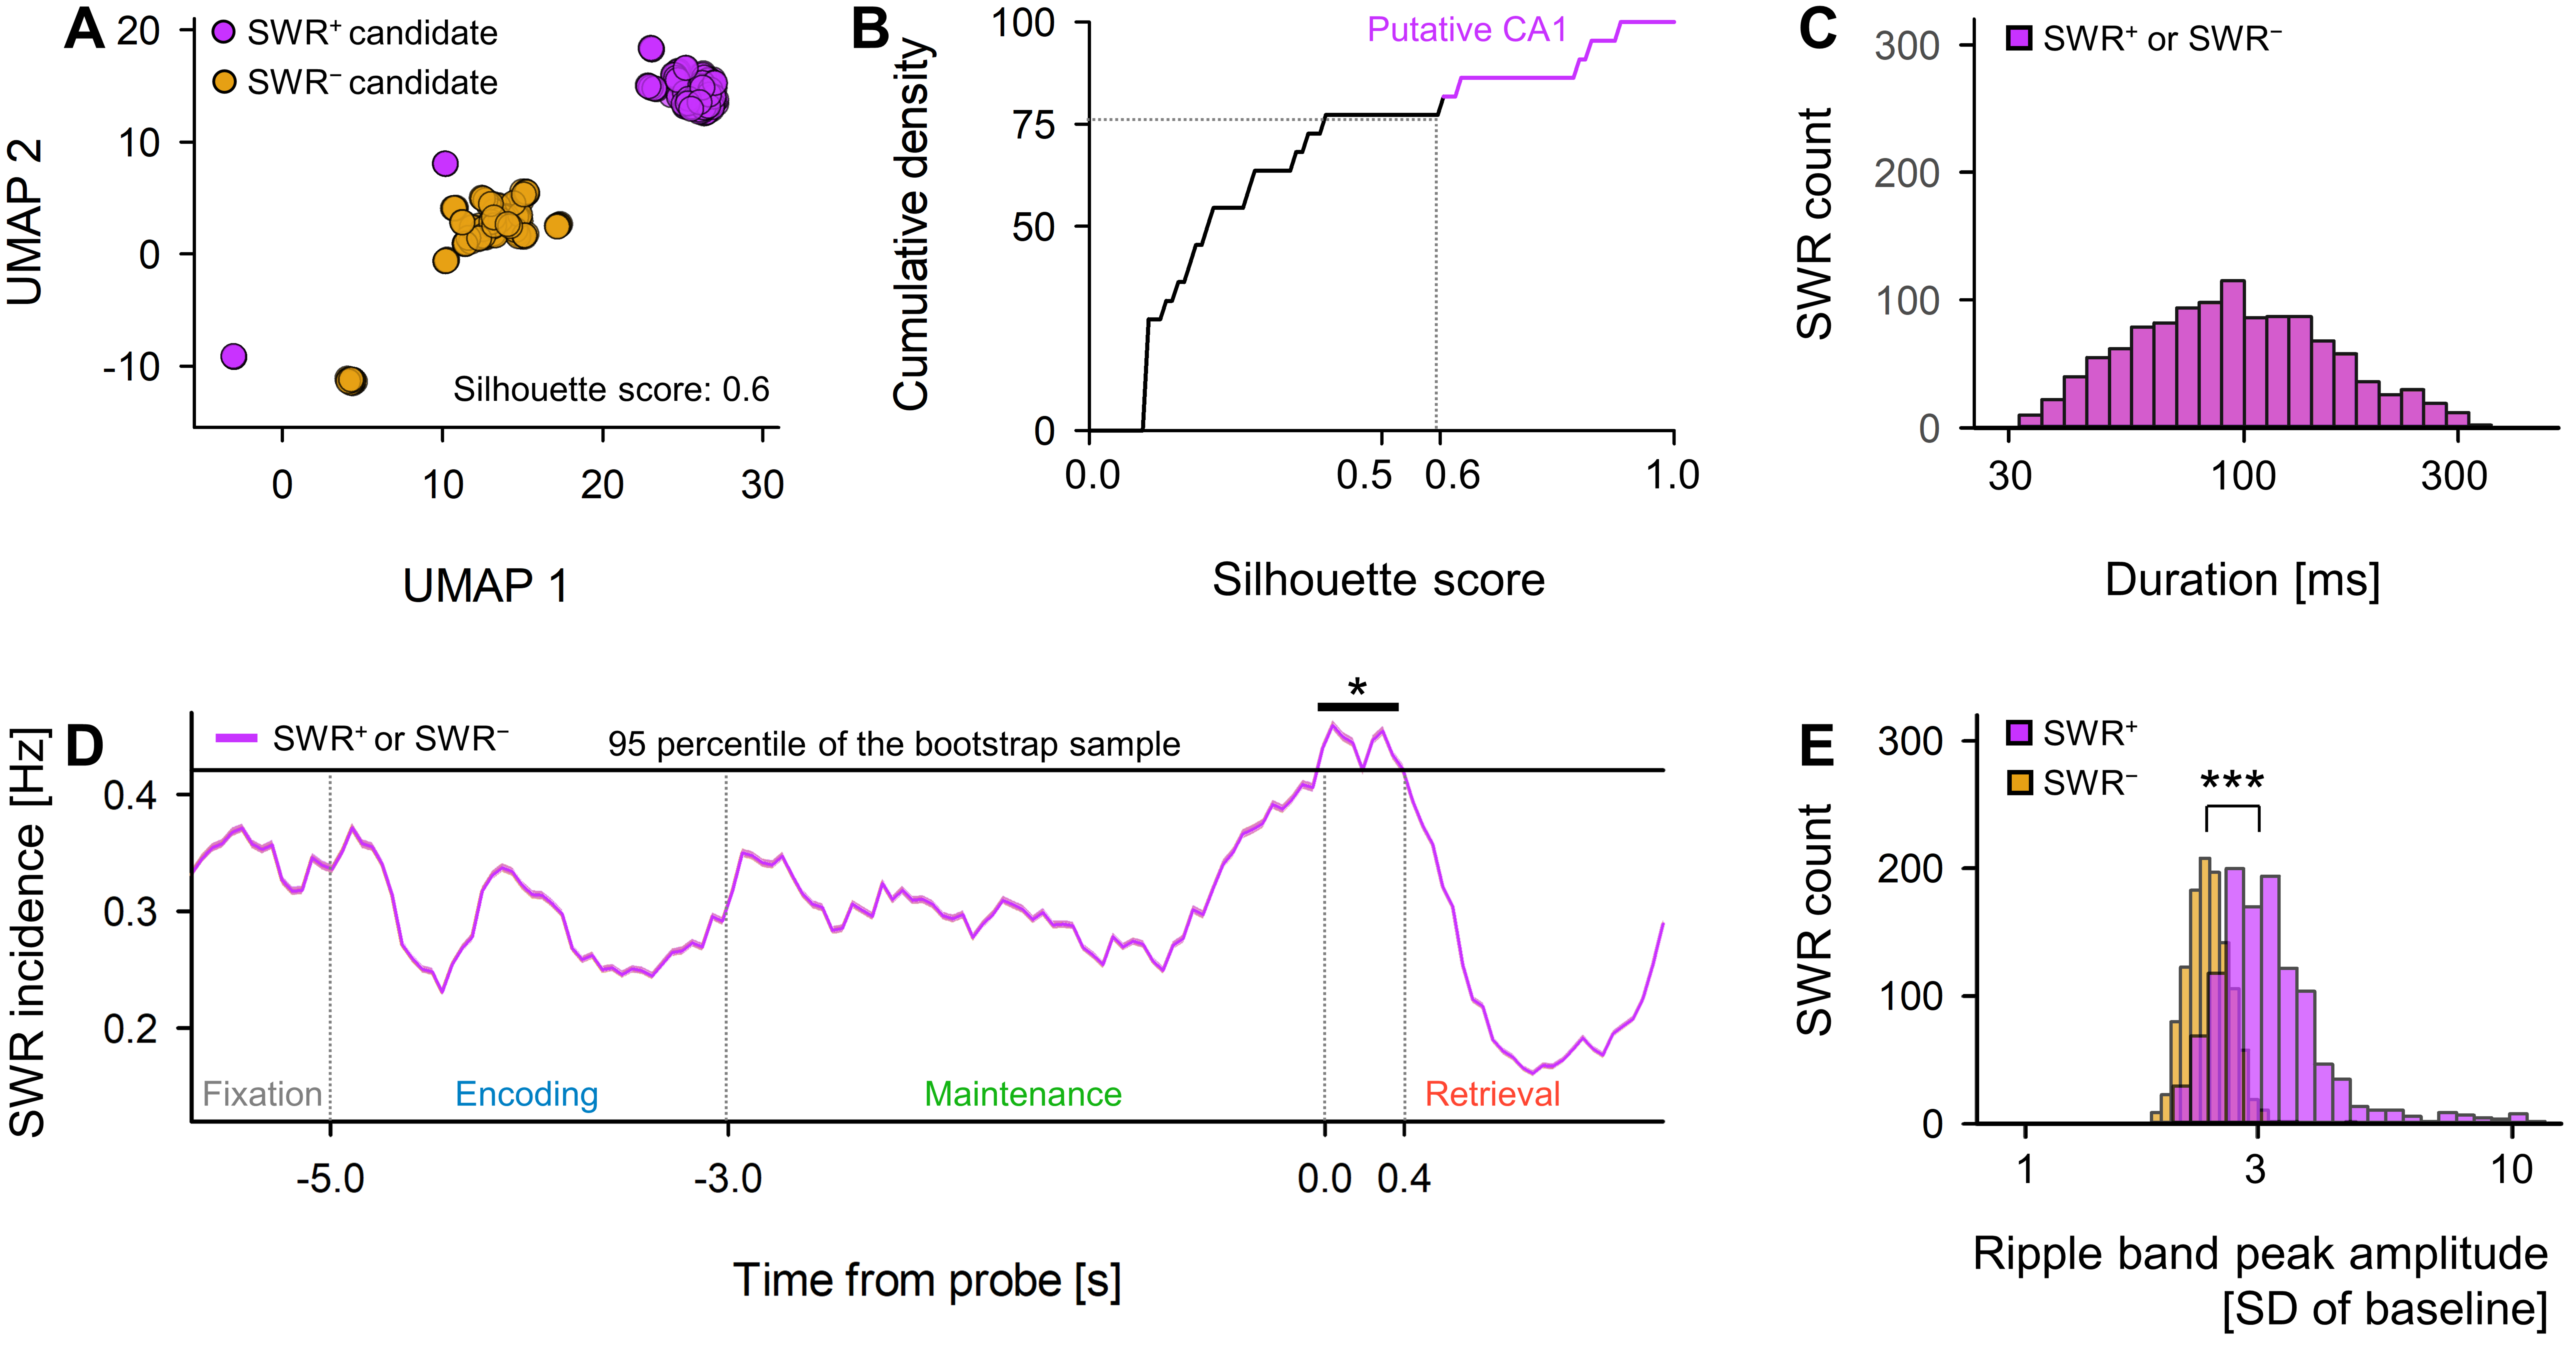
\includegraphics[width=1\textwidth]{./src/figures/.png/Figure_ID_04.png}
        	\caption{\textbf{Detection of SWRs in Putative CA1 Regions}\\
\textbf{\textit{A.}} Two-dimensional UMAP \cite{mcinnes_umap_2018} projection displays multi-unit spikes during SWR$^+$ candidates (\textit{purple}) and SWR$^-$ candidates (\textit{yellow}). \textbf{\textit{B.}} A cumulative density plot indicates silhouette scores, reflecting UMAP clustering quality (see Table~\ref{tab:02}). Hippocampal regions with silhouette scores exceeding 0.60 (equivalent to the $75^{th}$ percentile) are identified as putative CA1 regions. SWR$^+$ and SWR$^-$ candidates, which were recorded from these regions, are classified as SWR$^+$ and SWR$^-$ respectively (\textit{n}s = 1,170). \textbf{\textit{C.}} Identical distributions of durations are presented for SWR$^+$ (\textit{purple}) and SWR$^-$ (\textit{yellow}), based on their definitions (93.0 [65.4] ms, median [IQR]). \textbf{\textit{D.}} SWR incidence for both SWR$^+$ (\textit{purple}) and SWR$^-$ (\textit{yellow}), relative to the probe's timing, is illustrated as a mean \textpm 95\% confidence interval. However, intervals may not be visibly apparent due to their confined ranges, be aware that a significant SWR incidence increase was detected during the initial 400 ms of the retrieval phase (0.421 [Hz], *\textit{p} $<$ 0.05, bootstrap test). \textbf{\textit{E.}} Distributions of ripple band peak amplitudes for SWR$^-$ (\textit{yellow}; 2.37 [0.33] SD of baseline, median [IQR]) and SWR$^+$ (\textit{purple}; 3.05 [0.85] SD of baseline, median [IQR]) are manifested (***\textit{p} $<$ 0.001, the Brunner--Munzel test).}
% width=1\textwidth
        	\label{fig:04}
        \end{figure*}
